\documentclass[conference]{IEEEtran}
\IEEEoverridecommandlockouts
\usepackage{cite}
\usepackage{amsmath,amssymb,amsfonts}
\usepackage{graphicx}
\usepackage{textcomp}
\usepackage{xcolor}
\usepackage{booktabs}
\usepackage{multirow}
\usepackage[hidelinks]{hyperref}
\usepackage{url}

% auto-generated by src/analysis.py -- do not edit by hand
\newcommand{\NRuns}{213}
\newcommand{\TotalWh}{16.2}
\newcommand{\TotalG}{11.6}
\newcommand{\EnergyCpuRho}{0.99}
\newcommand{\CpuTdp}{8}
\newcommand{\RamW}{10}
\newcommand{\CarbonCv}{11}
\newcommand{\EqMargin}{5}
\newcommand{\PyVer}{3.13.18}
\newcommand{\VerNumpy}{2.5.3}
\newcommand{\VerPandas}{3.0.5}
\newcommand{\VerScikitLearn}{1.9.1}
\newcommand{\VerScipy}{1.18.1}
\newcommand{\VerMatplotlib}{3.11.2}
\newcommand{\VerCodecarbon}{3.3.1}
\newcommand{\VerOpenpyxl}{3.1.5}
\newcommand{\VerPsutil}{7.2.2}
\newcommand{\FraudAccBest}{HGB-HPO}
\newcommand{\FraudValBest}{RF-500}
\newcommand{\FraudGvp}{RF-100}
\newcommand{\FraudGvpCap}{73.1}
\newcommand{\FraudBestCap}{76.6}
\newcommand{\FraudGvpVcap}{74.4}
\newcommand{\FraudBestVcap}{76.7}
\newcommand{\FraudAccBestCap}{79.3}
\newcommand{\FraudHpoCap}{79.3}
\newcommand{\FraudGvpMg}{200}
\newcommand{\FraudHpoMg}{302}
\newcommand{\FraudBestMg}{1,026}
\newcommand{\FraudAccBestMg}{302}
\newcommand{\FraudSaveHpo}{33.7}
\newcommand{\FraudSaveBest}{80.5}
\newcommand{\FraudCarbonSpan}{1,737}
\newcommand{\FraudValueSpan}{27.0}
\newcommand{\FraudTestBestModel}{Linear}
\newcommand{\FraudTestBestCap}{83.9}
\newcommand{\FraudRhoCV}{-0.04}
\newcommand{\FraudRhoCVp}{0.91}
\newcommand{\FraudRhoCA}{+0.30}
\newcommand{\FraudRhoAV}{+0.73}
\newcommand{\FraudRhoAVp}{0.02}
\newcommand{\FraudRhoAVz}{-0.08}
\newcommand{\FraudDecGain}{27.9}
\newcommand{\FraudDecGainMean}{7.4}
\newcommand{\FraudModGain}{16.2}
\newcommand{\FraudModGainModel}{HGB-HPO}
\newcommand{\FraudNegDefault}{0}
\newcommand{\FraudSccShare}{$6.7{\times}10^{-8}$}
\newcommand{\FraudAccLoss}{-2.7}
\newcommand{\FraudAccBestAcc}{0.977}
\newcommand{\FraudBestAcc}{0.966}
\newcommand{\FraudAnnualKgIN}{0.06}
\newcommand{\FraudDTwoPct}{77}
\newcommand{\FraudCapDOne}{74.0}
\newcommand{\FraudCapDTwo}{77.1}
\newcommand{\FraudCapDTwoRaw}{73.0}
\newcommand{\FraudTostDiff}{-3.4}
\newcommand{\FraudTostLo}{-9.9}
\newcommand{\FraudTostHi}{0.6}
\newcommand{\FraudTostLoNinety}{-8.7}
\newcommand{\FraudTostHiNinety}{0.3}
\newcommand{\FraudTostEq}{no}
\newcommand{\FraudTostNi}{no}
\newcommand{\FraudTostHpoDiff}{-6.1}
\newcommand{\FraudTostHpoLo}{-13.4}
\newcommand{\FraudTostHpoHi}{2.3}
\newcommand{\FraudTostHpoLoNinety}{-12.4}
\newcommand{\FraudTostHpoHiNinety}{0.4}
\newcommand{\FraudTostHpoEq}{no}
\newcommand{\FraudTostHpoNi}{no}
\newcommand{\FraudBootAccDiff}{2.7}
\newcommand{\FraudBootAccLo}{-6.8}
\newcommand{\FraudBootAccHi}{10.9}
\newcommand{\FraudBootAccLoNinety}{-4.9}
\newcommand{\FraudBootAccHiNinety}{9.7}
\newcommand{\FraudBootAccEq}{no}
\newcommand{\FraudBootAccNi}{yes}
\newcommand{\ChurnAccBest}{HGB-HPO}
\newcommand{\ChurnValBest}{Linear}
\newcommand{\ChurnGvp}{Linear}
\newcommand{\ChurnGvpCap}{81.4}
\newcommand{\ChurnBestCap}{81.4}
\newcommand{\ChurnGvpVcap}{82.3}
\newcommand{\ChurnBestVcap}{82.3}
\newcommand{\ChurnAccBestCap}{81.6}
\newcommand{\ChurnHpoCap}{81.6}
\newcommand{\ChurnGvpMg}{$<$0.01}
\newcommand{\ChurnHpoMg}{148}
\newcommand{\ChurnBestMg}{$<$0.01}
\newcommand{\ChurnAccBestMg}{148}
\newcommand{\ChurnSaveHpo}{$>$99.9}
\newcommand{\ChurnSaveBest}{0.0}
\newcommand{\ChurnCarbonSpan}{$2.4{\times}10^{5}$}
\newcommand{\ChurnValueSpan}{1.9}
\newcommand{\ChurnTestBestModel}{HGB-HPO}
\newcommand{\ChurnTestBestCap}{81.6}
\newcommand{\ChurnRhoCV}{+0.30}
\newcommand{\ChurnRhoCVp}{0.40}
\newcommand{\ChurnRhoCA}{+0.22}
\newcommand{\ChurnRhoAV}{+0.76}
\newcommand{\ChurnRhoAVp}{0.01}
\newcommand{\ChurnRhoAVz}{+0.49}
\newcommand{\ChurnDecGain}{22.6}
\newcommand{\ChurnDecGainMean}{28.0}
\newcommand{\ChurnModGain}{0.0}
\newcommand{\ChurnModGainModel}{Linear}
\newcommand{\ChurnNegDefault}{0}
\newcommand{\ChurnSccShare}{$7.8{\times}10^{-13}$}
\newcommand{\ChurnAccLoss}{-0.2}
\newcommand{\ChurnAccBestAcc}{0.846}
\newcommand{\ChurnBestAcc}{0.844}
\newcommand{\ChurnAnnualKgIN}{0.00}
\newcommand{\ChurnDTwoPct}{86}
\newcommand{\ChurnCapDOne}{79.3}
\newcommand{\ChurnCapDTwo}{81.2}
\newcommand{\ChurnCapDTwoRaw}{80.8}
\newcommand{\ChurnTostHpoDiff}{-0.2}
\newcommand{\ChurnTostHpoLo}{-0.9}
\newcommand{\ChurnTostHpoHi}{0.7}
\newcommand{\ChurnTostHpoLoNinety}{-0.8}
\newcommand{\ChurnTostHpoHiNinety}{0.5}
\newcommand{\ChurnTostHpoEq}{yes}
\newcommand{\ChurnTostHpoNi}{yes}
\newcommand{\ChurnBootAccDiff}{0.2}
\newcommand{\ChurnBootAccLo}{-0.7}
\newcommand{\ChurnBootAccHi}{0.9}
\newcommand{\ChurnBootAccLoNinety}{-0.5}
\newcommand{\ChurnBootAccHiNinety}{0.8}
\newcommand{\ChurnBootAccEq}{yes}
\newcommand{\ChurnBootAccNi}{yes}
\newcommand{\CreditAccBest}{RF-100}
\newcommand{\CreditValBest}{RF-500}
\newcommand{\CreditGvp}{RF-500}
\newcommand{\CreditGvpCap}{11.1}
\newcommand{\CreditBestCap}{11.1}
\newcommand{\CreditGvpVcap}{16.7}
\newcommand{\CreditBestVcap}{16.7}
\newcommand{\CreditAccBestCap}{15.2}
\newcommand{\CreditHpoCap}{7.1}
\newcommand{\CreditGvpMg}{1.82}
\newcommand{\CreditHpoMg}{30}
\newcommand{\CreditBestMg}{1.82}
\newcommand{\CreditAccBestMg}{0.36}
\newcommand{\CreditSaveHpo}{93.9}
\newcommand{\CreditSaveBest}{0.0}
\newcommand{\CreditCarbonSpan}{$4.6{\times}10^{4}$}
\newcommand{\CreditValueSpan}{16.4}
\newcommand{\CreditTestBestModel}{RF-100}
\newcommand{\CreditTestBestCap}{15.2}
\newcommand{\CreditRhoCV}{+0.36}
\newcommand{\CreditRhoCVp}{0.31}
\newcommand{\CreditRhoCA}{+0.24}
\newcommand{\CreditRhoAV}{+0.56}
\newcommand{\CreditRhoAVp}{0.09}
\newcommand{\CreditRhoAVz}{-0.24}
\newcommand{\CreditDecGain}{89.2}
\newcommand{\CreditDecGainMean}{108.9}
\newcommand{\CreditModGain}{-1.0}
\newcommand{\CreditModGainModel}{HGB-100}
\newcommand{\CreditNegDefault}{10}
\newcommand{\CreditSccShare}{$1.9{\times}10^{-9}$}
\newcommand{\CreditAccLoss}{-4.1}
\newcommand{\CreditAccBestAcc}{0.770}
\newcommand{\CreditBestAcc}{0.773}
\newcommand{\CreditAnnualKgIN}{0.00}
\newcommand{\CreditDTwoPct}{57}
\newcommand{\CreditCapDOne}{7.4}
\newcommand{\CreditCapDTwo}{9.2}
\newcommand{\CreditCapDTwoRaw}{8.4}
\newcommand{\CreditTostHpoDiff}{4.0}
\newcommand{\CreditTostHpoLo}{-4.1}
\newcommand{\CreditTostHpoHi}{13.3}
\newcommand{\CreditTostHpoLoNinety}{-2.8}
\newcommand{\CreditTostHpoHiNinety}{11.7}
\newcommand{\CreditTostHpoEq}{no}
\newcommand{\CreditTostHpoNi}{yes}
\newcommand{\CreditBootAccDiff}{4.1}
\newcommand{\CreditBootAccLo}{-0.9}
\newcommand{\CreditBootAccHi}{10.0}
\newcommand{\CreditBootAccLoNinety}{-0.1}
\newcommand{\CreditBootAccHiNinety}{8.7}
\newcommand{\CreditBootAccEq}{no}
\newcommand{\CreditBootAccNi}{yes}
\newcommand{\RetailAccBest}{HGB-100}
\newcommand{\RetailValBest}{HGB-100}
\newcommand{\RetailGvp}{HGB-100}
\newcommand{\RetailGvpCap}{31.3}
\newcommand{\RetailBestCap}{31.3}
\newcommand{\RetailGvpVcap}{30.6}
\newcommand{\RetailBestVcap}{30.6}
\newcommand{\RetailAccBestCap}{31.3}
\newcommand{\RetailHpoCap}{31.3}
\newcommand{\RetailGvpMg}{1.35}
\newcommand{\RetailHpoMg}{176}
\newcommand{\RetailBestMg}{1.35}
\newcommand{\RetailAccBestMg}{1.35}
\newcommand{\RetailSaveHpo}{99.2}
\newcommand{\RetailSaveBest}{0.0}
\newcommand{\RetailCarbonSpan}{$7.0{\times}10^{5}$}
\newcommand{\RetailValueSpan}{31.5}
\newcommand{\RetailTestBestModel}{HGB-HPO}
\newcommand{\RetailTestBestCap}{31.3}
\newcommand{\RetailRhoCV}{+0.49}
\newcommand{\RetailRhoCVp}{0.13}
\newcommand{\RetailRhoCA}{+0.48}
\newcommand{\RetailRhoAV}{+0.99}
\newcommand{\RetailRhoAVp}{0.00}
\newcommand{\RetailRhoAVz}{+0.93}
\newcommand{\RetailDecGain}{0.6}
\newcommand{\RetailDecGainMean}{0.8}
\newcommand{\RetailModGain}{3.6}
\newcommand{\RetailModGainModel}{HGB-100}
\newcommand{\RetailNegDefault}{0}
\newcommand{\RetailSccShare}{$1.1{\times}10^{-9}$}
\newcommand{\RetailAccLoss}{0.0}
\newcommand{\RetailAccBestAcc}{0.661}
\newcommand{\RetailBestAcc}{0.661}
\newcommand{\RetailAnnualKgIN}{0.00}
\newcommand{\RetailTostHpoDiff}{0.0}
\newcommand{\RetailTostHpoLo}{-0.2}
\newcommand{\RetailTostHpoHi}{0.2}
\newcommand{\RetailTostHpoLoNinety}{-0.2}
\newcommand{\RetailTostHpoHiNinety}{0.2}
\newcommand{\RetailTostHpoEq}{yes}
\newcommand{\RetailTostHpoNi}{yes}
\newcommand{\AblHgbFive}{0.0}
\newcommand{\AblHgbFull}{69.5}
\newcommand{\AblHgbRatio}{2}
\newcommand{\AblRfFive}{75.2}
\newcommand{\AblRfFull}{73.1}
\newcommand{\AblRfRatio}{115}
\newcommand{\AblLinFive}{79.8}
\newcommand{\AblLinFull}{83.9}
\newcommand{\AblLinRatio}{15}

\newcommand{\RRValueBest}{Tree-d6}
\newcommand{\RRGvp}{Tree-d6}
\newcommand{\RRGvpSaving}{0.0}
\newcommand{\RRBestTest}{16.6}
\newcommand{\RRGvpTest}{16.6}

% auto-generated by src/sensitivity.py -- do not edit by hand
\newcommand{\SensN}{38}
\newcommand{\SensNinety}{6}
\newcommand{\SensWithin}{38}
\newcommand{\SensNinetyWithin}{6}
\newcommand{\SensSame}{25}
\newcommand{\SensWorst}{-3.4}
\newcommand{\SensMedianSave}{0}
\newcommand{\SensRhoMin}{-0.63}
\newcommand{\SensRhoMax}{+0.55}
\newcommand{\SensRhoMed}{+0.27}
\newcommand{\SensHpoBest}{3}
\newcommand{\SensHpoNinety}{35}
\newcommand{\SensHpoMedian}{99.8}
\newcommand{\SensHpoWithin}{36}
\newcommand{\SensBeatsHpo}{21}
\newcommand{\SensCoreN}{26}
\newcommand{\SensCoreNinety}{5}
\newcommand{\SensCoreMedian}{0}
\newcommand{\SensCreditDistinct}{1}
\newcommand{\SensRealN}{12}
\newcommand{\SensRealNinety}{1}
\newcommand{\SensRealMedian}{0.0}

\newcommand{\RepoURL}{\url{https://github.com/ashishhraj/Green-Value-ML}}

\begin{document}

\title{Beyond Accuracy: An Empirical Study of\\ Machine-Learning Carbon Emissions versus\\ Business Value Fulfilment}

\author{\IEEEauthorblockN{Ashish Raj, Ashwin Karthikeyan, Souvik Chakraborty}
\IEEEauthorblockA{\textit{Goa Institute of Management} \\
\textit{Big Data Analytics}\\
Student IDs: B2026065, B2026066, B2026104}}

\maketitle

\begin{abstract}
Green-AI evaluations report model carbon against accuracy, but firms are paid for decisions. We test whether extra
carbon buys extra business value in four decision problems: fraud screening, churn retention and credit approval on
public data, and perishable ordering on seeded synthetic data. A ten-rung model ladder (linear models to
hyper-parameter search) is trained over repeated splits (\NRuns{} runs); training and inference are metered separately
with CodeCarbon, and predictions are priced with explicit utility functions. Every choice---thresholds, probability
calibration, decision rule, value-best model and the \emph{Green Value Point} (GVP, the lowest-carbon model within 5\%
of the best validation value)---is made on validation data; the test set only reports outcomes and paired-bootstrap
equivalence (TOST) tests. Training emissions span three to six orders of magnitude, yet no domain shows a significant
carbon--value correlation, and hyper-parameter search is never the value-best model. In churn, credit and retail the
GVP uses \CreditSaveHpo\% to \ChurnSaveHpo\% less training carbon than the search and is equivalent to it within
$\pm$\EqMargin{} points of oracle value (churn, retail) or non-inferior (credit); fraud, with about 98 frauds per test
split, is inconclusive. The
decision rule outweighs the model: a calibrated, value-aware rule adds \ChurnDecGain{} to \CreditDecGain{} points in
three domains at sub-milligram cost, and only after this rule is applied does accuracy track value. A
\SensN{}-setting sensitivity analysis and a UCI Online Retail check bound these modeled, assumption-based results.
Absolute emissions are estimates from a TDP-based power model.
\end{abstract}

\begin{IEEEkeywords}
Green AI, carbon footprint, business value, cost-sensitive learning, model selection, sustainable machine learning
\end{IEEEkeywords}

\section{Introduction}
Organisations increasingly report the environmental footprint of their digital operations, and ML is a visible part of
it~\cite{strubell2019,kaack2022}. In the EU, the Corporate Sustainability Reporting Directive requires in-scope firms to
disclose energy use and greenhouse-gas emissions~\cite{csrd2022}, so the compute behind models becomes a reportable cost.
The Green-AI movement~\cite{schwartz2020} asks practitioners to report energy and carbon next to model quality, and a
growing toolset makes this measurable~\cite{lacoste2019,henderson2020,codecarbon,eco2ai}. In almost all of this work,
however, ``quality'' means accuracy, F1 or perplexity~\cite{verdecchia2023}. A manager does not bank accuracy. A fraud
model can rank transactions well and still lose money if it flags many small ones that cost more to investigate than they
are worth. The question that matters to a business is therefore: \emph{does spending more carbon on a model buy more
business value?}

We hypothesise that the carbon--accuracy trade-off documented in Green-AI studies overstates the
carbon--\emph{value} trade-off, because (i) business value saturates earlier than accuracy and (ii) much of the value
is created downstream of the model, in the decision rule that turns scores into actions.

\subsection{Scope and Objectives}
We study four tabular decision problems, the bulk of industrial ML~\cite{grinsztajn2022}, and ask:
\begin{itemize}
\item \textbf{RQ1:} Is more training carbon associated with more business value?
\item \textbf{RQ2:} Does the accuracy ranking of models predict their value ranking?
\item \textbf{RQ3:} Is value created mainly by the model or by the decision rule, and at what carbon cost?
\item \textbf{RQ4:} How material is carbon in money terms once a model is deployed, and how robust are the conclusions?
\end{itemize}
Our contributions are: (1) a unified, example-dependent utility framework that prices predictions from four domains in
one equation; (2) a benchmark of \NRuns{} metered runs on three public and one synthetic dataset, plus a real
transaction-data check; (3) the GVP and \emph{value capture} metrics, with a validation-only selection protocol and
equivalence tests that certify (or fail to certify) a low-carbon choice; and (4) evidence that decision-rule design,
including a probability-quality check before a Bayes rule is used, dominates model scale as a source of value per gram
of CO$_2$e.

\section{Related Work}
\textbf{Carbon of ML.} Strubell \emph{et al.}~\cite{strubell2019} quantified the emissions of training NLP models;
Schwartz \emph{et al.}~\cite{schwartz2020} proposed efficiency as an evaluation criterion. Lacoste \emph{et
al.}~\cite{lacoste2019} and Henderson \emph{et al.}~\cite{henderson2020} gave methods for systematic reporting, and
Patterson \emph{et al.}~\cite{patterson2021} and Luccioni \emph{et al.}~\cite{luccioni2023,luccioni2024} measured large
models end-to-end, showing that inference can dominate lifetime energy. Wu \emph{et al.}~\cite{wu2022} framed
sustainability across the ML life cycle, and Verdecchia \emph{et al.}~\cite{verdecchia2023} found that most Green-AI
studies trade energy against accuracy-type metrics only. Recent multi-objective work searches for energy--accuracy
Pareto fronts in architecture search~\cite{ecnas2024}, hyper-parameter tuning~\cite{ecopt2026} and model
selection~\cite{betello2025}; the performance axis is still accuracy.

\textbf{Value of ML.} Cost-sensitive learning~\cite{elkan2001} and example-dependent costs~\cite{bahnsen2015} recognise
that errors differ in price. Profit-driven evaluation is mature in churn~\cite{verbeke2012,verbraken2013,hoppner2020}
and credit scoring, and the newsvendor model links forecasts to inventory cost.

\textbf{Gap.} Table~\ref{tab:gap} positions our work. Carbon studies ignore money; profit studies ignore carbon; neither
separates the model from the decision rule. We join the two lines across four domains.

\begin{table}[t]
\centering
\caption{Positioning against prior work.}
\label{tab:gap}
\scriptsize
\setlength{\tabcolsep}{1.5pt}
\resizebox{\columnwidth}{!}{%
\begin{tabular}{lcccc}
\toprule
Work & Carbon & Money value & Domains & Decision rule \\ \midrule
Green AI~\cite{strubell2019,schwartz2020,luccioni2024} & \checkmark & -- & several & -- \\
Energy--accuracy Pareto~\cite{ecnas2024,ecopt2026,betello2025} & \checkmark & -- & several & -- \\
Profit-driven~\cite{verbraken2013,hoppner2020,bahnsen2015} & -- & \checkmark & one & partly \\
\textbf{This study} & \checkmark & \checkmark & four & \checkmark \\
\bottomrule
\end{tabular}
}
\end{table}

\section{Methodology}
\subsection{Data}
Table~\ref{tab:data} summarises the settings. \emph{Fraud}: 284,807 European card transactions with 492 frauds
(0.17\%)~\cite{dalpozzolo2015}. \emph{Churn}: 7,043 IBM Telco customers, 26.5\% churners~\cite{ibmtelco}. \emph{Credit}:
the 1,000-applicant Statlog German credit data, 30\% defaults~\cite{hofmann1994}. \emph{Retail}: a generated panel of 120
perishable SKUs over three years with trend, weekly and yearly seasonality, promotions with price elasticity, festival
peaks and over-dispersed negative-binomial demand (seed 2026). For a real transaction-data check we use UCI Online
Retail~\cite{uciretail}: 541,909 invoice lines are aggregated to daily demand for the 120 products with the highest
first-half sales; cancelled invoices and non-positive quantities/prices are removed and zero-sale days kept. The data
contain no inventory, unit cost or spoilage, so unit cost is assumed to be 60\% of each product's first-half median
price and holding cost 30\% of unit cost; this is modeled cost avoided, not observed profit. Preprocessing: one-hot
encoding, blank \texttt{TotalCharges} set to zero, $\log(1{+}\text{amount})$ and hour-of-day for fraud, and leakage-free
lag and rolling features for retail. Classification uses stratified 60/20/20 train/validation/test splits repeated over 3
seeds (fraud), 5 (churn) and 10 (credit, being small); synthetic retail uses a fixed chronological split (seeds vary
model randomness only); UCI retail uses three rolling-origin folds.

\begin{table}[t]
\centering
\caption{Scenarios and value definitions (vs.\ doing nothing).}
\label{tab:data}
\scriptsize
\setlength{\tabcolsep}{2.5pt}
\resizebox{\columnwidth}{!}{%
\begin{tabular}{llrl}
\toprule
Scenario & Source & Rows & Action and value \\ \midrule
Fraud & ULB~\cite{dalpozzolo2015} & 284,807 & review: amount caught $-$ \texteuro5/alert \\
Churn & IBM~\cite{ibmtelco} & 7,043 & offer: $0.3{\times}12{\times}$monthly $-$ \$25/offer \\
Credit & Statlog~\cite{hofmann1994} & 1,000 & approve: 10\% margin, 60\% LGD \\
Retail & synthetic & 128,040 & order: newsvendor cost saved \\
UCI retail & Online Retail~\cite{uciretail} & 41,520 & demand: assumed inventory cost (\pounds) \\
\bottomrule
\end{tabular}
}
\end{table}

\subsection{A Unified Business-Value Framework}
For the three classification problems, a model's score $p_i$ triggers an action (review, offer, reject). The value of a
policy that acts on the set $\mathcal{F}$ is
\begin{equation}
V(\mathcal{F}) = c_0 + \sum_{i\in\mathcal{F}} \big[\, y_i\,P_i - (1-y_i)\,N_i \,\big],
\label{eq:value}
\end{equation}
where $P_i$ is the example-dependent gain of acting on a true positive, $N_i$ the cost of acting on a false positive and
$c_0$ the value of doing nothing. For fraud, $P_i = a_i - r$ and $N_i = r$, with amount $a_i$ and review cost
$r$=\texteuro5. For churn, $P_i = \gamma H m_i - f$ and $N_i = f$, with acceptance $\gamma$=0.3, horizon $H$=12 months,
monthly charge $m_i$ and offer cost $f$=\$25, following the EMPC logic~\cite{verbraken2013}. For credit, rejecting a loan avoids
$P_i=\ell a_i$ (LGD $\ell$=0.6) and forgoes $N_i = \mu a_i$ (margin $\mu$=0.1); $c_0$ is the value of approving all. The
perfect-foresight oracle earns $V^\star = c_0 + \sum_{y_i=1}\max(P_i,0)$ and we report \emph{value capture}
$100\,V/V^\star$, comparable across currencies and domains. For retail, an order $q_{it}$ for demand $d_{it}$
costs $h\,u_i(q_{it}{-}d_{it})^+ + (s_{it}{-}u_i)(d_{it}{-}q_{it})^+$ (spoilage at $h$=30\% of unit cost $u_i$, lost
margin at price $s_{it}$); value is the cost saved against ordering last week's sales.

\subsection{Model Ladder and Decision Rules}
Each scenario uses the same ten rungs, ordered by compute: logistic/ridge regression (\emph{Linear}), a depth-6 tree,
random forests with 100 and 500 trees, histogram gradient boosting (HGB) with 100 and 500 iterations, MLPs with one
(64) and three (256-256-128) hidden layers, a stacked ensemble (RF-100, HGB-100, MLP-S, logistic meta-learner) and
HGB-HPO, a 20-candidate, 3-fold randomised search. Retail adds a seasonal-naive reference. Every prediction is priced under
three rules: \textbf{D0}, the default $p_i \geq 0.5$ (or order = forecast); \textbf{D1}, one threshold (or order uplift
$\alpha$) tuned on validation to maximise~(\ref{eq:value}); and \textbf{D2}, the example-dependent Bayes rule
\begin{equation}
\text{act on } i \iff \hat p_i P_i > (1-\hat p_i) N_i,
\label{eq:bayes}
\end{equation}
applied to probabilities $\hat p_i$ that have passed a probability-quality check. Raw scores of trees, forests and MLPs
need not be probabilities, so before D2 is used we measure the Brier score and ten-bin expected calibration error (ECE)
on validation, fit Platt scaling~\cite{platt1999} on the validation scores (cross-fitted in two folds so that no
validation row is calibrated by itself), re-measure ECE, and apply the fitted calibrator unchanged to test. Because the
probabilities are calibrated, (\ref{eq:bayes}) is used with no tuned scale factor~\cite{elkan2001,bahnsen2015}. The
\emph{value-aware} rule is whichever of D1/D2 has the higher cross-fitted validation value. For comparison we also log
the earlier rule that tuned a scale factor $\lambda$ on raw scores (D2$_\text{raw}$); it is never used for selection.

\subsection{Carbon Measurement and Its Uncertainty}\label{sec:carbon}
Training and inference are metered separately with CodeCarbon~\cite{codecarbon} in offline mode on the Indian grid
(0.713\,kg CO$_2$e/kWh) on a 2-vCPU Intel Xeon (2.1\,GHz, 7.8\,GB RAM) with \texttt{n\_jobs}=2 for all models. A warm-up
fit precedes each scenario so that start-up overheads are not billed to the first model; inference is repeated until it
lasts $\geq$2\,s and reported per 1,000 predictions. \emph{How energy is estimated.} The virtual machine exposes no RAPL
energy counters and its CPU is not in CodeCarbon's database, so CodeCarbon assigns a default thermal design power (TDP)
of 4\,W per thread (\CpuTdp\,W) and each second estimates CPU power as $\text{TDP}\,(0.1+0.9L^3)$, with $L$ the machine CPU
load, plus a constant \RamW\,W for memory; energy is this power integrated over wall-clock time. Two consequences follow.
First, estimated energy is nearly proportional to runtime, so its agreement with process CPU-seconds (Spearman
$\rho$=\EnergyCpuRho) is partly by construction and supports only relative comparisons. Second, the absolute level rests
on assumed wattages: memory is 56--93\% of estimated power, and a true CPU TDP between 0.5$\times$ and 3$\times$ the
default would shift full-load power by about $-$22\% to $+$89\%. Run-to-run spread is smaller (median relative s.d.\ of
training emissions across splits \CarbonCv\%), so Table~\ref{tab:carbonparts} reports training and inference separately
with that spread, but we treat absolute grams as indicative. Conclusions rest on rankings, ratios and on business value,
which is deterministic given the seeds.

\subsection{Selection Protocol and Statistics}
All choices are made on validation data: the D1 threshold, the D2 calibrator, the D1/D2 choice, the value-best model
(highest mean validation capture), the accuracy-best model (highest mean validation ROC-AUC, or 1$-$WAPE for retail), the
best model at the 0.5 rule and the \emph{Green Value Point} (GVP), the lowest-carbon model whose mean validation capture
is within 5\% of the best. The test set only reports the outcome of these choices; a unit test checks that changing test
labels cannot change any choice. Paired differences between two models are bootstrapped by resampling test rows
within each split (2,000 resamples) and averaging the difference in percentage points (pp) of oracle value over splits.
We then apply two one-sided tests (TOST)~\cite{schuirmann1987}: the GVP is \emph{equivalent} to a comparator if the 90\%
CI lies inside $\pm$\EqMargin\,pp and \emph{non-inferior} if its lower bound exceeds $-$\EqMargin\,pp. Spearman
correlations over the 10--11 models are descriptive: with so few models they have little power. The sensitivity
analysis follows the same protocol, and a life-cycle projection (Sec.~\ref{sec:lifecycle}) combines training and
inference under an explicitly hypothetical deployment profile.

\section{Results}
\begin{table*}[t]
\centering
\caption{Model ladder results (mean over repeated splits). C = training emissions in mg CO$_2$e (CodeCarbon, Indian grid). Acc = test ROC-AUC (retail: 1$-$WAPE). V$_{0.5}$ / V$^{\ast}$ = test business value captured as \% of the perfect-foresight oracle under the default 0.5 rule / the value-aware rule. Bold = value-best, \underline{underline} = accuracy-best and $\dagger$ = Green Value Point, all three \emph{selected on validation data}; the test columns only report their outcome.}
\label{tab:ladder}
\scriptsize
\setlength{\tabcolsep}{3.2pt}
\begin{tabular}{lrrrrrrrrrrrrrrrr}
\toprule
 & \multicolumn{4}{c}{Fraud detection} & \multicolumn{4}{c}{Churn retention} & \multicolumn{4}{c}{Credit approval} & \multicolumn{4}{c}{Perishable ordering} \\
\cmidrule(lr){2-5}\cmidrule(lr){6-9}\cmidrule(lr){10-13}\cmidrule(lr){14-17}
Model & C & Acc & V$_{0.5}$ & V$^{\ast}$ & C & Acc & V$_{0.5}$ & V$^{\ast}$ & C & Acc & V$_{0.5}$ & V$^{\ast}$ & C & Acc & V$_{0.5}$ & V$^{\ast}$ \\ \midrule
Naive & -- & -- & -- & -- & -- & -- & -- & -- & -- & -- & -- & -- & $<$0.01 & 0.506 & 0.0 & -0.2 \\
Linear & 0.59 & 0.981 & 55.9 & 83.9 & $<$0.01 & 0.844 & 58.8 & \textbf{81.4}$^\dagger$ & $<$0.01 & 0.773 & -85.2 & 4.0 & $<$0.01 & 0.639 & 26.5 & 27.1 \\
Tree-d6 & 11 & 0.874 & 78.6 & 79.3 & $<$0.01 & 0.807 & 50.9 & 79.6 & $<$0.01 & 0.706 & -89.4 & -1.2 & 0.55 & 0.647 & 27.8 & 28.7 \\
RF-100 & 200 & 0.956 & 76.4 & 73.1$^\dagger$ & 0.69 & 0.836 & 51.0 & 81.0 & 0.36 & \underline{0.770} & -117.7 & 15.2 & 94 & 0.653 & 29.4 & 30.1 \\
RF-500 & 1,026 & 0.966 & 76.4 & \textbf{76.6} & 3.34 & 0.838 & 50.7 & 81.0 & 1.82 & 0.773 & -121.2 & \textbf{11.1}$^\dagger$ & 472 & 0.654 & 29.7 & 30.4 \\
HGB-100 & 1.83 & 0.863 & 67.2 & 69.5 & 0.88 & 0.830 & 52.5 & 80.6 & 0.54 & 0.762 & -86.2 & 13.8 & 1.35 & \underline{0.661} & 30.1 & \textbf{31.3}$^\dagger$ \\
HGB-500 & 1.93 & 0.822 & 55.7 & 56.8 & 6.36 & 0.812 & 48.9 & 80.6 & 2.61 & 0.758 & -84.3 & 10.5 & 2.70 & 0.660 & 30.1 & 31.2 \\
MLP-S & 13 & 0.967 & 60.8 & 82.7 & 0.52 & 0.836 & 53.2 & 81.0 & 0.10 & 0.709 & -118.8 & 2.6 & 17 & 0.658 & 29.5 & 30.6 \\
MLP-L & 129 & 0.964 & 80.8 & 83.4 & 5.47 & 0.829 & 57.3 & 81.2 & 0.61 & 0.772 & -100.8 & 12.3 & 83 & 0.657 & 29.8 & 30.9 \\
Stack & 575 & 0.978 & 68.8 & 82.6 & 7.29 & 0.843 & 52.5 & 81.0 & 3.57 & 0.775 & -106.3 & 12.4 & 331 & 0.659 & 30.2 & 30.9 \\
HGB-HPO & 302 & \underline{0.977} & 72.2 & 79.3 & 148 & \underline{0.846} & 53.2 & 81.6 & 30 & 0.753 & -91.3 & 7.1 & 176 & 0.661 & 30.2 & 31.3 \\
\midrule
Spearman $\rho$(C,V$^{\ast}$) & \multicolumn{4}{c}{-0.04 (p=0.91)} & \multicolumn{4}{c}{+0.30 (p=0.40)} & \multicolumn{4}{c}{+0.36 (p=0.31)} & \multicolumn{4}{c}{+0.49 (p=0.13)} \\
Spearman $\rho$(Acc,V$^{\ast}$) & \multicolumn{4}{c}{+0.73 (p=0.02)} & \multicolumn{4}{c}{+0.76 (p=0.01)} & \multicolumn{4}{c}{+0.56 (p=0.09)} & \multicolumn{4}{c}{+0.99 (p=0.00)} \\
\bottomrule
\end{tabular}
\end{table*}


\subsection{RQ1: More Carbon Buys Little Value}
Fig.~\ref{fig:cv} and Table~\ref{tab:ladder} show the core result. Training emissions span \FraudCarbonSpan-fold
(fraud) to \RetailCarbonSpan-fold (retail) across the learned models, yet no domain shows a significant carbon--value
rank correlation ($\rho$ from \FraudRhoCV{} in fraud to \RetailRhoCV{} in retail). The paired tests in
Table~\ref{tab:tost} are more informative. In churn, the validation-selected value-best model and GVP is Linear
(\ChurnGvpMg\,mg), equivalent to the search (\ChurnHpoMg\,mg) within $\pm$\EqMargin\,pp ($\Delta$V=\ChurnTostHpoDiff\,pp,
90\% CI [\ChurnTostHpoLoNinety, \ChurnTostHpoHiNinety]). In retail, HGB-100 (\RetailGvpMg\,mg) is both value-best and GVP
and matches the search (\RetailHpoMg\,mg) to within 0.2\,pp. In credit, RF-500 is value-best and GVP; it is non-inferior
to the search at \CreditSaveHpo\% less carbon, but split-to-split s.d.\ reaches 19\,pp, so equivalence is not shown.
In fraud, the GVP (RF-100) saves \FraudSaveBest\% of RF-500's training carbon at \FraudTostDiff\,pp, but the 90\% CI
reaches \FraudTostLoNinety\,pp: with about 98 frauds per test split, fraud value is too noisy to certify a
\EqMargin-pp margin. Fraud also shows why selection must stay off the test set: the cheap Linear model has the highest
test capture (\FraudTestBestCap\%) but ranked below RF-500 on validation, so a test-selected analysis would have called
it the value-best model. Hyper-parameter search was the validation value-best model in none of the four domains.

\begin{figure*}[t]
\centering
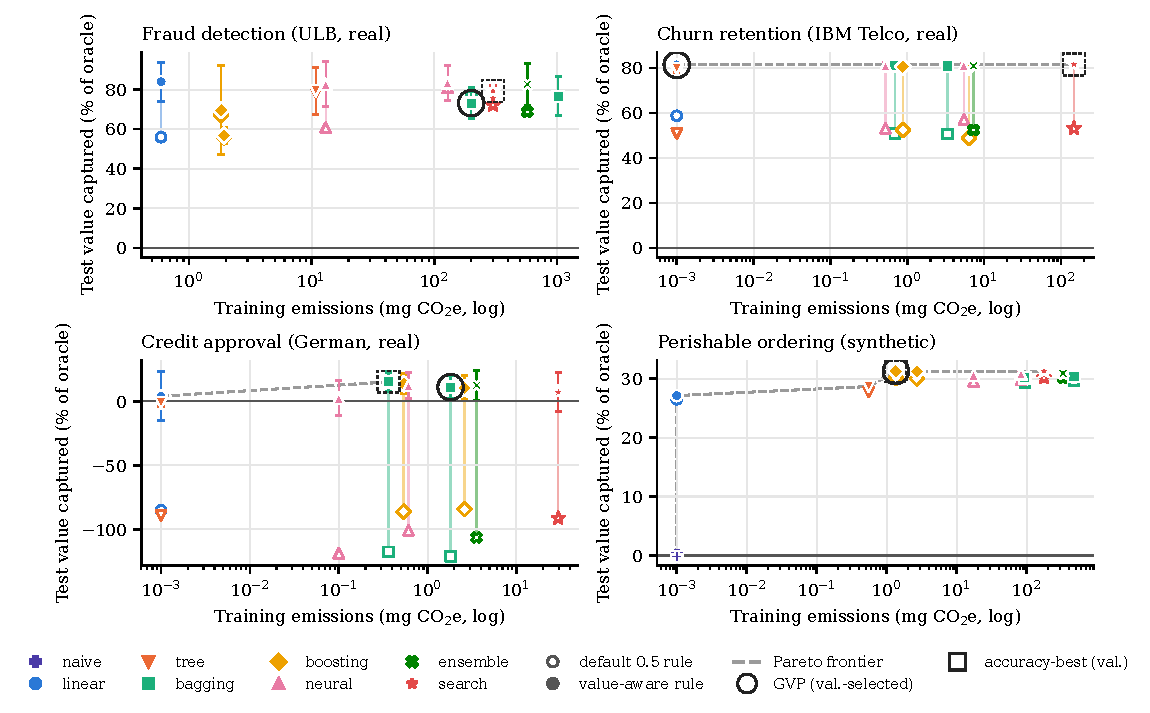
\includegraphics[width=\textwidth]{figures/fig_carbon_value.pdf}
\caption{Training emissions (log scale) vs.\ test business value captured, mean $\pm$ s.d.\ over splits. Hollow markers:
default 0.5 rule; filled: value-aware rule; thin vertical lines join the two for each model. Circle: Green Value Point;
dashed square: accuracy-best model (both selected on validation).}
\label{fig:cv}
\end{figure*}

\begin{table}[t]
\centering
\caption{Test-set check of the validation-selected Green Value Point (GVP) against the validation-selected value-best model (when different) and against hyper-parameter search (HGB-HPO). $\Delta$V = GVP $-$ comparator in pp of oracle value, mean over splits, paired bootstrap (2,000 resamples). TOST: equivalent if the 90\% CI lies inside $\pm$5 pp. NI = non-inferior (lower 90\% bound $>-$5 pp).}
\label{tab:tost}
\scriptsize
\setlength{\tabcolsep}{2.2pt}
\begin{tabular}{lllrrrcc}
\toprule
Scen. & GVP & vs. & C saved & $\Delta$V & 90\% CI & TOST & NI \\ \midrule
Fraud & RF-100 & RF-500 & 80\% & -3.4 & [-8.7, +0.3] & no & no \\
 &  & HGB-HPO & 34\% & -6.1 & [-12.4, +0.4] & no & no \\
Churn & Linear & HGB-HPO & $>$99.9\% & -0.2 & [-0.8, +0.5] & yes & yes \\
Credit & RF-500 & HGB-HPO & 94\% & +4.0 & [-2.8, +11.7] & no & yes \\
Retail & HGB-100 & HGB-HPO & 99\% & 0.0 & [-0.2, +0.2] & yes & yes \\
\bottomrule
\end{tabular}
\end{table}


\subsection{RQ2: Accuracy Tracks Value Only After the Decision Is Priced}
The validation accuracy-best model differs from the value-best model in three of four domains (fraud, churn, credit),
but the test differences are small and not significant (fraud \FraudBootAccDiff\,pp, 95\% CI [\FraudBootAccLo,
\FraudBootAccHi]; credit \CreditBootAccDiff\,pp [\CreditBootAccLo, \CreditBootAccHi]). More revealing is how the
accuracy--value relation depends on the decision layer. At the default 0.5 rule, ROC-AUC rank is unrelated to value in
fraud ($\rho$=\FraudRhoAVz) and credit (\CreditRhoAVz) and weak in churn (\ChurnRhoAVz); under the value-aware rule
(Fig.~\ref{fig:av}) it rises to \FraudRhoAV, \CreditRhoAV{} and \ChurnRhoAV. Accuracy is therefore a reasonable proxy
for value only once the decision has been priced; retail, with near-symmetric costs, tracks value under both rules
($\rho$=\RetailRhoAVz{} and \RetailRhoAV).

\begin{figure}[t]
\centering
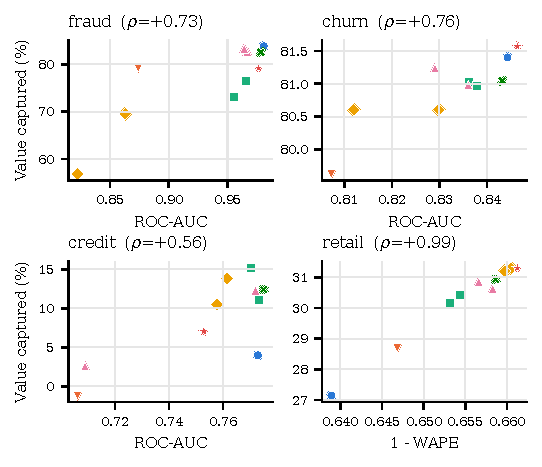
\includegraphics[width=\columnwidth]{figures/fig_acc_value.pdf}
\caption{Test accuracy vs.\ value capture per model under the value-aware rule; $\rho$ is the Spearman correlation.
Markers as in Fig.~\ref{fig:cv}.}
\label{fig:av}
\end{figure}

\subsection{RQ3: The Decision Rule Beats the Model}
Table~\ref{tab:layers} decomposes value into a model upgrade (Linear$\rightarrow$the model with the best validation
value at the 0.5 rule) and a decision upgrade (Linear, 0.5 rule$\rightarrow$value-aware rule, whose tuning and
calibration were themselves metered). In credit, all \CreditNegDefault{} models \emph{lose} money at the 0.5 cut-off,
because a 30\% default rate with a 6:1 loss-to-margin ratio puts the break-even probability at $\mu/(\mu{+}\ell)\approx$0.14,
not 0.5. The decision upgrade adds \CreditDecGain\,pp for a fraction of a microgram, against \CreditModGain\,pp for the
model upgrade. In churn the decision upgrade adds \ChurnDecGain\,pp and no model beats Linear at 0.5; in fraud it adds
\FraudDecGain\,pp at 0.4\,mg, against \FraudModGain\,pp for HGB-HPO at \FraudHpoMg\,mg. Retail, whose costs are symmetric
enough for the plain forecast to be near-optimal, gains more from the model. In three of four domains the cheapest
lever to pull first is the decision rule.

\begin{table}[t]
\centering
\caption{Where the business value comes from (test, pp of oracle value; C in mg CO$_2$e). Model upgrade = Linear$\rightarrow$the model with the best \emph{validation} value at the 0.5 rule. Decision upgrade = Linear, 0.5 rule$\rightarrow$value-aware rule (C = metered cost of tuning and calibrating the rule).}
\label{tab:layers}
\scriptsize
\setlength{\tabcolsep}{2.6pt}
\begin{tabular}{llrrrr}
\toprule
 & \multicolumn{3}{c}{Model upgrade} & \multicolumn{2}{c}{Decision upgrade} \\
\cmidrule(lr){2-4}\cmidrule(lr){5-6}
Scenario & to & $\Delta$V & $\Delta$C & $\Delta$V & $\Delta$C \\ \midrule
Fraud & HGB-HPO & +16.2 & 301 & +27.9 & 0.52 \\
Churn & Linear & 0.0 & $<$0.01 & +22.6 & $<$0.01 \\
Credit & HGB-100 & -1.0 & 0.54 & +89.2 & $<$0.01 \\
Retail & HGB-100 & +3.6 & 1.35 & +0.6 & $<$0.01 \\
\bottomrule
\end{tabular}
\end{table}


Table~\ref{tab:calibration} reports the probability check made before D2 is used. Raw scores are poorly calibrated for
some churn and credit models (worst-model ECE up to 0.18); Platt scaling fitted on validation lowers mean ECE on
validation and, with the calibrator frozen, on test. (Fraud ECE is near zero only because 99.8\% of cases are
legitimate, so it says little.) The calibrated Bayes rule won the validation comparison in \FraudDTwoPct\% (fraud),
\ChurnDTwoPct\% (churn) and \CreditDTwoPct\% (credit) of runs. Averaged over all runs, its test capture
(\FraudCapDTwo, \ChurnCapDTwo{} and \CreditCapDTwo\%) exceeds both the tuned threshold D1 (\FraudCapDOne, \ChurnCapDOne,
\CreditCapDOne\%) and the earlier $\lambda$-tuned raw-score rule (\FraudCapDTwoRaw, \ChurnCapDTwoRaw, \CreditCapDTwoRaw\%).

\begin{table}[t]
\centering
\caption{Probability quality, checked on validation before the Bayes rule D2 is used. ECE (ten bins) of raw scores and of Platt-calibrated probabilities (cross-fitted on validation; calibrator then applied unchanged to test). Mean over all runs, worst model mean in brackets. D2 = share of runs in which the calibrated Bayes rule beat the tuned threshold on validation and was therefore used.}
\label{tab:calibration}
\scriptsize
\setlength{\tabcolsep}{2.2pt}
\begin{tabular}{lrrrrr}
\toprule
 & \multicolumn{2}{c}{Validation ECE} & \multicolumn{2}{c}{Test ECE} & \\
\cmidrule(lr){2-3}\cmidrule(lr){4-5}
Scenario & raw & calibrated & raw & calibrated & D2 used \\ \midrule
Fraud & 0.001 [0.002] & 0.000 [0.000] & 0.001 [0.001] & 0.000 [0.000] & 77\% \\
Churn & 0.044 [0.111] & 0.029 [0.052] & 0.040 [0.111] & 0.029 [0.051] & 86\% \\
Credit & 0.100 [0.184] & 0.063 [0.087] & 0.095 [0.176] & 0.070 [0.094] & 57\% \\
\bottomrule
\end{tabular}
\end{table}


\subsection{Real Transaction-Data Check}
Table~\ref{tab:retailreal} reports the UCI Online Retail panel. The model and the GVP are chosen on each fold's
validation window and capture is measured on the later test window. The validation value-best model, \RRValueBest, is
also the GVP and captures \RRBestTest\% of oracle value on test. The heavier models (forests, the stack and the search)
are unstable on this lumpy demand, with near-zero or negative mean capture and fold-to-fold s.d.\ above 20\,pp, so the real data
agree that more carbon does not buy value. The monetary proxy rests on assumed unit and holding costs, so this is a
check on transaction-derived demand, not evidence of realised savings.

\begin{table}[t]
\centering
\caption{UCI Online Retail (real transactions), three rolling-origin folds. The value-best model (bold) and the GVP ($\dagger$) are selected on each fold's validation window; capture is then reported on the later test window (mean $\pm$ s.d.\ over folds). C = training emissions (mg CO$_2$e). Value uses an assumed cost proxy.}
\label{tab:retailreal}
\scriptsize
\setlength{\tabcolsep}{3pt}
\begin{tabular}{lrrrr}
\toprule
Model & C & $1-$WAPE & Val.\ capture (\%) & Test capture (\%) \\ \midrule
Naive & 0 & -0.171 & 3.0 $\pm$ 0.4 & 2.4 $\pm$ 0.8 \\
Linear & 0.15 & -0.148 & 8.3 $\pm$ 3.5 & 6.9 $\pm$ 1.4 \\
\textbf{Tree-d6}$^\dagger$ & 0.23 & 0.022 & 17.0 $\pm$ 3.0 & 16.6 $\pm$ 2.0 \\
RF-100 & 52 & -0.921 & -7.1 $\pm$ 37.2 & -7.5 $\pm$ 35.5 \\
RF-500 & 258 & -0.764 & -1.8 $\pm$ 30.0 & -2.3 $\pm$ 27.8 \\
HGB-100 & 0.89 & -0.184 & 11.2 $\pm$ 8.0 & 10.3 $\pm$ 6.3 \\
HGB-500 & 1.3 & -0.138 & 10.6 $\pm$ 5.8 & 9.2 $\pm$ 4.8 \\
MLP-S & 4.1 & 0.054 & 11.4 $\pm$ 3.1 & 8.2 $\pm$ 1.7 \\
MLP-L & 19 & 0.027 & 11.8 $\pm$ 2.8 & 8.7 $\pm$ 2.2 \\
Stack & 151 & -0.658 & 0.9 $\pm$ 24.6 & 0.5 $\pm$ 22.3 \\
HGB-HPO & 148 & -0.907 & -7.8 $\pm$ 44.0 & -10.2 $\pm$ 40.9 \\
\bottomrule
\end{tabular}
\end{table}


\subsection{Data Volume}
Fig.~\ref{fig:abl} retrains three fraud models on 5--100\% of the training set. Training carbon of RF-100 grows
\AblRfRatio$\times$ while its value capture stays flat (\AblRfFive\% at 5\%, \AblRfFull\% at 100\%); Linear moves from
\AblLinFive\% to \AblLinFull\%. HGB with default settings is unstable at 0.17\% prevalence at every size, a reminder that
variance across splits can exceed the differences between models.

\begin{figure}[t]
\centering
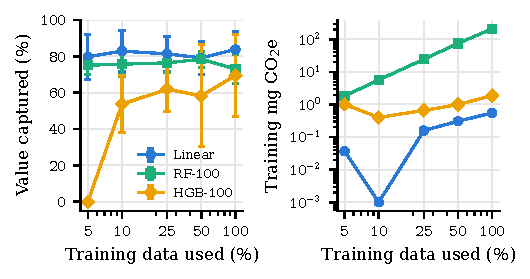
\includegraphics[width=\columnwidth]{figures/fig_ablation.pdf}
\caption{Fraud data-volume ablation: value capture (left) and training emissions (right) vs.\ share of training data used.}
\label{fig:abl}
\end{figure}

\subsection{RQ4: Life-Cycle Carbon and Its Price}\label{sec:lifecycle}
We illustrate annual operation with stated workload assumptions: fraud retrained weekly and scoring 100\,M transactions;
churn retrained monthly with one campaign over 1\,M customers; credit retrained quarterly for 100k applications; retail
retrained weekly for 1,000 SKUs forecast daily. Measured per-run training emissions are multiplied by the retraining
count and measured per-1,000 batch-inference emissions by the prediction volume; serving overheads, idle capacity, data
pipelines, networking and embodied hardware emissions are excluded, so these are lower-bound operational estimates, not
deployment logs. Table~\ref{tab:carbonparts} keeps training and inference separate. Training dominates where retraining
is frequent (fraud, retail); inference dominates for the rarely retrained churn and credit models. Even the largest
footprint, fraud's RF-500, is about 59\,g CO$_2$e per year on the Indian grid, and moving to the French grid cuts every
figure by a factor of 13. Priced at the US EPA social cost of carbon (\$190/t)~\cite{epa2023}, carbon is below
$10^{-7}$\% of the modeled value in every domain. For tabular decision models, carbon is therefore not material in money
terms; the case for the GVP rests on statistical sufficiency, simplicity and auditability, not on carbon cost.

\begin{table}[t]
\centering
\caption{Projected annual footprint of the value-best (B) and GVP (G) models under the illustrative deployment profile of Sec.~\ref{sec:lifecycle}, in g CO$_2$e on the Indian grid: training and inference shown separately as mean ($\pm$ relative s.d.\ across repeated runs: run-to-run metering spread only; see Sec.~\ref{sec:carbon} for the larger power-model uncertainty). FR = total on the French grid. SCC = social cost of carbon (\$190/t) as a share of the model's annual modeled value.}
\label{tab:carbonparts}
\scriptsize
\setlength{\tabcolsep}{2pt}
\resizebox{\columnwidth}{!}{%
\begin{tabular}{llrrrr}
\toprule
Scen. & Model & Training & Inference & FR & SCC/value \\ \midrule
Fraud & B: RF-500 & 53 ($\pm$4\%) & 5.6 ($\pm$7\%) & 4.6 & $6.7{\times}10^{-8}$\% \\
 & G: RF-100 & 10 ($\pm$4\%) & 1 ($\pm$7\%) & 0.9 & $1.4{\times}10^{-8}$\% \\
Churn & B: Linear & $7.4{\times}10^{-6}$ ($\pm$14\%) & $2.2{\times}10^{-3}$ ($\pm$16\%) & $1.7{\times}10^{-4}$ & $7.8{\times}10^{-13}$\% \\
Credit & B: RF-500 & $7.3{\times}10^{-3}$ ($\pm$7\%) & 0.12 ($\pm$9\%) & $9.8{\times}10^{-3}$ & $1.9{\times}10^{-9}$\% \\
Retail & B: HGB-100 & 0.07 ($\pm$3\%) & $1.3{\times}10^{-3}$ ($\pm$4\%) & $5.6{\times}10^{-3}$ & $1.1{\times}10^{-9}$\% \\
\bottomrule
\end{tabular}}
\end{table}


\subsection{Robustness to Business Assumptions}
We re-priced all saved predictions under \SensN{} alternative cost settings (fraud review cost \texteuro2--20; churn
acceptance 0.15--0.5 $\times$ offer cost \$10--50; credit margin 0.05--0.2 $\times$ LGD 0.4--0.8; synthetic-retail spoilage
10--100\%; real-retail unit cost 40--80\% of reference price $\times$ holding cost 10--100\%). In each setting the decision
rules are re-tuned, the rule is re-chosen and the value-best model and GVP are re-selected on validation; the test set is
used only to report the outcome. In all \SensWithin{} of \SensN{} settings the GVP's test value was within
\EqMargin\,pp of the validation value-best model (worst \SensWorst\,pp), and in \SensHpoWithin{} of \SensN{} within
\EqMargin\,pp of HGB-HPO, while using at least 90\% less training carbon than the search in \SensHpoNinety{} (median
saving \SensHpoMedian\%). The search was the value-best model in only \SensHpoBest{} settings. Savings relative to the
value-best model are usually zero (median \SensMedianSave\%) because in \SensSame{} settings the value-best model was
itself the GVP, typically a cheap model. In credit the value-best model was RF-500 in all nine settings. In the
real-retail grid the value-best model was always Tree-d6 or MLP-S, both cheap, and the GVP beat the search on test in all
\SensRealN{} settings.

\section{Discussion}
\textbf{Relevance and significance.} For a firm that must report its digital footprint, the results give a simple
order of work: \emph{price the decision, check and calibrate the probabilities, tune the rule, then scale the model only
while validation value improves.} In this benchmark, hyper-parameter search never paid for itself, the decision rule
added more value than any model upgrade in three of four domains, and the low-carbon GVP was certified as equivalent or
non-inferior in three domains. These are modeled outcomes under stated utility functions, not observed profits or causal
campaign effects.

\textbf{Contribution.} Prior studies relate carbon to accuracy~\cite{strubell2019,schwartz2020,ecopt2026} or value to
accuracy~\cite{verbraken2013,hoppner2020}; this benchmark combines carbon and modeled decision value across four domains,
separates the model and decision layers, and shows that the accuracy--value link depends on the decision layer. It is a
cross-domain integration; we do not claim a first-in-literature result.

\textbf{Limitations.} We study CPU-scale tabular models; deep models may have a different carbon curve. Absolute
emissions come from an assumed-TDP power model (Sec.~\ref{sec:carbon}). Utilities are assumptions, and campaign effects
are omitted. Fraud and credit value are noisy: the fraud GVP could not be certified at a 5-pp margin, and validation sets
of 200 credit applicants make selection unstable. Synthetic retail is generated, and the transaction check covers one
retailer without inventory, cost or spoilage records. Deployment workloads are illustrative.

\section{Reproducibility}
Code, run configurations, run-level results, validation and test predictions, figures and the LaTeX source are
available at \RepoURL{} (MIT licence). All datasets except the 100\,MB fraud file are in the repository; that file is
fetched and checksummed by \texttt{src/download\_data.py}, and synthetic data are regenerated with seed 2026.
\texttt{make reproduce} re-runs the study (about 75 minutes on two CPU cores here); \texttt{make analysis} regenerates
every table, figure and in-text number from the saved predictions in minutes, and \texttt{make test} runs unit tests for
the value functions and for the no-test-leakage protocol. Every number in this paper is a macro written by the scripts.
\texttt{results/run\_config.json} records the hardware, the CodeCarbon power model, all seeds and business parameters,
and the versions used: Python \PyVer, scikit-learn \VerScikitLearn, pandas \VerPandas, NumPy \VerNumpy, SciPy
\VerScipy{} and CodeCarbon \VerCodecarbon. Re-running a model reproduces its test value exactly; carbon figures vary
with hardware and load.

\subsection{AI Use Declaration}
AI tools (Anthropic Claude and OpenAI ChatGPT) were used for idea scoping, initial code scaffolding and revision,
language editing and LaTeX formatting. All experimental design decisions, analysis and interpretation were reviewed by
the authors, and AI-generated content (text or code) constitutes less than 20\% of the submission, as verified by
Turnitin.

\section{Conclusion}
Across fraud, churn, credit and two retail settings, additional training carbon did not buy significantly more modeled
business value. With every choice made on validation data, a low-carbon Green Value Point matched hyper-parameter search
in churn and retail, was non-inferior in credit and remained inconclusive in fraud. A calibrated, value-aware decision
rule added more value than model scale at negligible compute, and it is also what makes accuracy a useful guide to
value. Prospective validation on operational data with real cost records is the next step before treating the GVP as
deployment guidance.

\section*{Acknowledgment}
The authors thank \emph{the course instructor} for guidance, and the maintainers of the ULB, IBM and UCI datasets and of
CodeCarbon.

\begin{thebibliography}{00}
\bibitem{strubell2019} E. Strubell, A. Ganesh, and A. McCallum, ``Energy and policy considerations for deep learning in NLP,'' in \emph{Proc. 57th Annu. Meeting Assoc. Comput. Linguistics (ACL)}, Florence, Italy, 2019, pp. 3645--3650.
\bibitem{kaack2022} L. H. Kaack, P. L. Donti, E. Strubell, G. Kamiya, F. Creutzig, and D. Rolnick, ``Aligning artificial intelligence with climate change mitigation,'' \emph{Nature Climate Change}, vol. 12, pp. 518--527, 2022.
\bibitem{csrd2022} European Parliament and Council of the European Union, ``Directive (EU) 2022/2464 as regards corporate sustainability reporting (CSRD),'' \emph{Official Journal of the European Union}, L 322, Dec. 2022.
\bibitem{schwartz2020} R. Schwartz, J. Dodge, N. A. Smith, and O. Etzioni, ``Green AI,'' \emph{Commun. ACM}, vol. 63, no. 12, pp. 54--63, 2020.
\bibitem{lacoste2019} A. Lacoste, A. Luccioni, V. Schmidt, and T. Dandres, ``Quantifying the carbon emissions of machine learning,'' arXiv:1910.09700, 2019.
\bibitem{henderson2020} P. Henderson, J. Hu, J. Romoff, E. Brunskill, D. Jurafsky, and J. Pineau, ``Towards the systematic reporting of the energy and carbon footprints of machine learning,'' \emph{J. Mach. Learn. Res.}, vol. 21, no. 248, pp. 1--43, 2020.
\bibitem{codecarbon} B. Courty \emph{et al.}, ``CodeCarbon: Track emissions from compute,'' Zenodo, 2024. [Online]. Available: https://github.com/mlco2/codecarbon
\bibitem{eco2ai} S. A. Budennyy \emph{et al.}, ``eco2AI: Carbon emissions tracking of machine learning models as the first step towards sustainable AI,'' \emph{Doklady Mathematics}, vol. 106, suppl. 1, pp. S118--S128, 2022.
\bibitem{verdecchia2023} R. Verdecchia, J. Sallou, and L. Cruz, ``A systematic review of Green AI,'' \emph{WIREs Data Mining Knowl. Discov.}, vol. 13, no. 4, e1507, 2023.
\bibitem{grinsztajn2022} L. Grinsztajn, E. Oyallon, and G. Varoquaux, ``Why do tree-based models still outperform deep learning on typical tabular data?'' in \emph{Adv. Neural Inf. Process. Syst. (NeurIPS) Datasets and Benchmarks Track}, 2022.
\bibitem{patterson2021} D. Patterson \emph{et al.}, ``Carbon emissions and large neural network training,'' arXiv:2104.10350, 2021.
\bibitem{luccioni2023} A. S. Luccioni, S. Viguier, and A.-L. Ligozat, ``Estimating the carbon footprint of BLOOM, a 176B parameter language model,'' \emph{J. Mach. Learn. Res.}, vol. 24, no. 253, pp. 1--15, 2023.
\bibitem{luccioni2024} A. S. Luccioni, Y. Jernite, and E. Strubell, ``Power hungry processing: Watts driving the cost of AI deployment?'' in \emph{Proc. ACM Conf. Fairness, Accountability, and Transparency (FAccT)}, 2024.
\bibitem{wu2022} C.-J. Wu \emph{et al.}, ``Sustainable AI: Environmental implications, challenges and opportunities,'' in \emph{Proc. Mach. Learn. Syst. (MLSys)}, 2022.
\bibitem{ecnas2024} P. Bakhtiarifard, C. Igel, and R. Selvan, ``EC-NAS: Energy consumption aware tabular benchmarks for neural architecture search,'' arXiv:2210.06015, 2024.
\bibitem{ecopt2026} E. Dos Santos Ferreira, N. D. Lawrence, and A. Paleyes, ``Optimising for energy efficiency and performance in machine learning,'' arXiv:2601.08991, 2026.
\bibitem{betello2025} F. Betello and A. Purificato, ``One search fits all: Pareto-optimal eco-friendly model selection,'' arXiv:2505.01468, 2025.
\bibitem{elkan2001} C. Elkan, ``The foundations of cost-sensitive learning,'' in \emph{Proc. 17th Int. Joint Conf. Artif. Intell. (IJCAI)}, 2001, pp. 973--978.
\bibitem{bahnsen2015} A. Correa Bahnsen, D. Aouada, and B. Ottersten, ``Example-dependent cost-sensitive decision trees,'' \emph{Expert Syst. Appl.}, vol. 42, no. 19, pp. 6609--6619, 2015.
\bibitem{platt1999} J. C. Platt, ``Probabilistic outputs for support vector machines and comparisons to regularized likelihood methods,'' in \emph{Advances in Large Margin Classifiers}, A. J. Smola \emph{et al.}, Eds. Cambridge, MA, USA: MIT Press, 1999, pp. 61--74.
\bibitem{schuirmann1987} D. J. Schuirmann, ``A comparison of the two one-sided tests procedure and the power approach for assessing the equivalence of average bioavailability,'' \emph{J. Pharmacokinet. Biopharm.}, vol. 15, no. 6, pp. 657--680, 1987.
\bibitem{verbeke2012} W. Verbeke, K. Dejaeger, D. Martens, J. Hur, and B. Baesens, ``New insights into churn prediction in the telecommunication sector: A profit driven data mining approach,'' \emph{Eur. J. Oper. Res.}, vol. 218, no. 1, pp. 211--229, 2012.
\bibitem{verbraken2013} T. Verbraken, W. Verbeke, and B. Baesens, ``A novel profit maximizing metric for measuring classification performance of customer churn prediction models,'' \emph{IEEE Trans. Knowl. Data Eng.}, vol. 25, no. 5, pp. 961--973, 2013.
\bibitem{hoppner2020} S. H\"oppner, E. Stripling, B. Baesens, S. vanden Broucke, and T. Verdonck, ``Profit driven decision trees for churn prediction,'' \emph{Eur. J. Oper. Res.}, vol. 284, no. 3, pp. 920--933, 2020.
\bibitem{dalpozzolo2015} A. Dal Pozzolo, O. Caelen, R. A. Johnson, and G. Bontempi, ``Calibrating probability with undersampling for unbalanced classification,'' in \emph{Proc. IEEE Symp. Ser. Comput. Intell. (SSCI)}, 2015, pp. 159--166.
\bibitem{ibmtelco} IBM, ``Telco customer churn sample dataset,'' 2019. [Online]. Available: https://github.com/IBM/telco-customer-churn-on-icp4d
\bibitem{hofmann1994} H. Hofmann, ``Statlog (German Credit Data),'' UCI Machine Learning Repository, 1994. [Online]. Available: https://doi.org/10.24432/C5NC77
\bibitem{uciretail} D. Chen, ``Online Retail,'' UCI Machine Learning Repository, 2015. [Online]. Available: https://doi.org/10.24432/C5BW33
\bibitem{epa2023} U.S. Environmental Protection Agency, ``Report on the social cost of greenhouse gases: Estimates incorporating recent scientific advances,'' Washington, DC, USA, 2023.
\end{thebibliography}

\end{document}
